\documentclass[a4paper,11pt]{article}%Schriftgröße
\usepackage[T1]{fontenc} 
\renewcommand{\familydefault}{\sfdefault}
\usepackage[utf8]{inputenc}
\usepackage[ngerman]{babel}%Veröffentlichungssprache
\usepackage{graphicx}
\usepackage{ragged2e}
\usepackage[format=plain,justification=RaggedRight,singlelinecheck=false,font={small},labelsep=space]{caption}
\usepackage{xcolor}	
\usepackage[a4paper]{geometry}
\geometry{left=3.5cm,right=2.5cm,top=2.4cm,bottom=2cm}%Seitenränder
\usepackage[onehalfspacing]{setspace}%Zeilenabstand
\renewcommand{\\}{\vspace*{0.5\baselineskip} \newline}
\renewcommand*\MakeUppercase[1]{#1}	
\usepackage{fancyhdr}
\pagestyle{fancy}
\renewcommand{\headrulewidth}{0pt}
\renewcommand{\footrulewidth}{0pt}
\fancyhead[R]{\footnotesize{\thepage}}
\fancyhead[L]{\footnotesize{\leftmark}}
\fancyfoot{}
\usepackage[authoryear]{natbib}
\usepackage[colorlinks,
pdfpagelabels,
pdfstartview = FitH,
bookmarksopen = true,
bookmarksnumbered = true,
linkcolor = black,
urlcolor = black,
plainpages = false,
hypertexnames = false,
citecolor = black] {hyperref}
\usepackage[printonlyused, withpage, smaller]{acronym}

\begin{document}
	\begin{titlepage}
		\begin{flushleft}
			\vspace*{-1cm}
			
\includegraphics[scale=1]{Abbildungen/TH.png}\\
			\vspace*{1cm}
		\end{flushleft}
		\begin{huge}
			\noindent
			%Vergleich des Teambuildingerfolgs mittels eines nicht-vollkörpergetracktem- und vollkörpergetracktem Avatars in einer Immersive Virtual Reality anhand einer Escape-Room-Artigen Umgebung. \\
			
			Vertrauensaufbau einer Teambuildingmaßnahme zwischen eines Hand- und Kopf getracktem Avatar und  eines Hand-, Kopf und Inverskinematisch-simuliertem Torsos getracktem Avatar in einem Shared Virtual Environment anhand einer Escape-Room-Artigen Umgebung. \\
		\end{huge}
		Masterarbeit zur Erlangung des Master-Grades \newline
		\textit{Master of Science} im Studiengang Medientechnologie \newline
		an der Fakultät für Informations-, Medien- und Elektrotechnik \newline
		der Technischen Hochschule Köln \\
		~\\
		~\\
		~\\
		\noindent\begin{tabular}{ll}
			vorgelegt von: & Hannes Hinrichs \\
			Matrikel-Nr.: &	11121733 \\
			Adresse: & Zülpicher Straße 19 \\
			~ &	50987 Köln \\
			~ &	hannes.hinrichs@web.de \\
			~ & ~ \\
			eingereicht bei: & Prof. Dr. Arnulph Fuhrmann \\
			Zweitgutachter/in: & --------------------
		\end{tabular}	
		~\\
		~\\
		Ort, TT.MM.JJJJ
	\end{titlepage}
	\pagenumbering{Roman}
	\pagestyle{fancy}
	\newpage
	\section*{Erklärung}\markboth{Erklärung}{Erklärung}\addcontentsline{toc}{section}{Erklärung}
	Ich versichere, die von mir vorgelegte Arbeit selbstständig verfasst zu haben. Alle Stellen, die wörtlich oder sinngemäß aus veröffentlichten oder nicht veröffentlichten Arbeiten anderer oder der Verfasserin/des Verfassers selbst entnommen sind, habe ich als entnommen kenntlich gemacht. Sämtliche Quellen und Hilfsmittel, die ich für die Arbeit benutzt habe, sind angegeben. Die Arbeit hat mit gleichem Inhalt bzw. in wesentlichen Teilen noch keiner anderen Prüfungsbehörde vorgelegen.\\
	Anmerkung: In einigen Studiengängen steht die Erklärung am Ende des Textes.\\
	~\\
	~\\
	\rule{0.35\textwidth}{0.4pt} \hspace*{3cm} \rule{0.45\textwidth}{0.4pt} \newline
	Ort, Datum	\hspace*{6.3cm}	Rechtsverbindliche Unterschrift
	\newpage
	\section*{Kurzfassung/Abstract}\markboth{Kurzfassung/Abstract}{Kurzfassung/Abstract}\addcontentsline{toc}{section}{Kurzfassung/Abstract}
	Eine Kurzfassung (wenn verlangt) in Deutsch und/oder in Englisch (Abstract) umfasst auf etwa 1/2 bis 1 Seite die Darstellung der Problemstellung, der angewandten Methode(n) und des wichtigsten Ergebnisses.\\
	Wie man ein gelungenes Abstract verfasst, erfahren Sie in den \href{https://www.th-koeln.de/studium/schluesselkompetenzen_25490.php}{\underline{Seminaren des Akademischen} \underline{Schreibzentrums der Kompetenzwerkstatt}}.\\
	Schlagwörter/Schlüsselwörter: evtl. Angabe von 3 bis 10 Schlagwörtern 
	\newpage
	\tableofcontents
	\newpage
	
	\section*{Abkürzungsverzeichnis}\markboth{Abkürzungsverzeichnis}{Abkürzungsverzeichnis}\addcontentsline{toc}{section}{Abkürzungsverzeichnis}
	\begin{acronym}[NIK-T.Lvl.Rounds]
	\acro{hmd}[HMD]{Head-Mounted-Display}
	\acro{sve}[SVE]{Shared-Virtual-Environment}
	\acro{vr}[VR]{Virtual-Reality}
	\acro{ivr}[IVR]{Immersive-Virtual-Reality}
	\acro{ipo}[IPO]{Input-Process-Output}
	\acro{fov}[FOV]{Field-of-View}
	\acro{bip}[BIP]{Break-in-Presence}
	
	\acro{ik}[IK]{Invers-Kinematisch - (Hand-, Kopf und Inverskinematisch-simulierter Torso)}
	\acro{nik}[NIK]{Nicht-Invers-Kinematisch (Hand- und Kopf getrackter Avatar)}
	
	\acro{gt}[GT]{Generelles Vertrauen}
	\acro{gti}[GTI]{Generelles Vertrauen - IK}
	\acro{gtn}[GTN]{Generelles Vertrauen - NIK}
	
	\acro{ct}[CT]{Kognitives Vertrauen}
	\acro{cti}[CTI]{Kognitives Vertrauen - IK}
	\acro{ctn}[CTN]{Kognitives Vertrauen - NIK}
	
	\acro{tc}[TC]{Team-Kommunikation}
	\acro{tci}[TCI]{Team-Kommunikation - IK}
	\acro{tcn}[TCN]{Team-Kommunikation - NIK}
	
	\acro{tRound}[T.Lvl.Rounds]{Erfolgreich abgeschlossene Runden auf Team-Level}
	\acro{tRoundIK}[IK-T.Lvl.Rounds]{Erfolgreiche abgeschlossene Runden auf Team-Level - IK}
	\acro{tRoundNIK}[NIK-T.Lvl.Rounds]{Erfolgreiche abgeschlossene Runden auf Team-Level - NIK}
	
	\acro{te}[TE]{Teameffektivität}
	\acro{tei}[TEI]{Teameffektivität - IK}
	\acro{ten}[TEN]{Teameffektivität - NIK}
	
	\acro{cp}[CP]{Co-Präsenz}
	\acro{cpi}[CPI]{Co-Präsenz - IK}
	\acro{cpn}[CPN]{Co-Präsenz - NIK}
	
	\acro{tlx}[NTLX]{Nasa-TLX}
	\acro{tlxi}[NTLXI]{Nasa-TLX - IK}
	\acro{tlxn}[NTLXN]{Nasa-TLX - NIK}
	
	\acro{teamCog}[T.Lvl.Cog]{Kognitives Vertrauen auf Team-Level}
	\acro{teamCogIK}[IK-T.Lvl.Cog]{Kognitives Vertrauen auf Team-Level - IK}
	\acro{teamCogNIK}[NIK-T.Lvl.Cog]{Kognitives Vertrauen auf Team-Level - NIK}
	
	\acro{teamGen}[T.Lvl.Gen]{Generelles Vertrauen auf Team-Level}
	\acro{teamGenIK}[IK-T.Lvl.Gen]{Generelles Vertrauen auf Team-Level - IK}
	\acro{teamGenNIK}[NIK-T.Lvl.Gen]{Generelles Vertrauen auf Team-Level - NIK}
	
	\acro{scp}[SCP]{Self-Co-Präsenz}
	\acro{scpi}[SCPI]{Self-Co-Präsenz - IK}
	\acro{scpn}[SCPN]{Self-Co-Präsenz - NIK}	
	
	\acro{ocp}[OCP]{Other-Co-Präsenz}
	\acro{ocpi}[OCPI]{Other-Co-Präsenz - IK}
	\acro{ocpn}[OCPN]{Other-Co-Präsenz - NIK}	
	
	\acro{ipq}[IPQ]{Fragebogen des Anstrengungsmaß}
	\acro{ipqi}[IPQI]{Fragebogen des Anstrengungsmaß - IK}
	\acro{ipqn}[IPQN]{Fragebogen des Anstrengungsmaß - NIK}
	
	\acro{tp}[TP]{Telepresence}
	\acro{tpi}[TPI]{Telepresence - IK}
	\acro{tpn}[TPN]{Telepresence - NIK}	
	
	\acro{sp}[SP]{Social-Presence}
	\acro{spi}[SPI]{Social-Presence - IK}
	\acro{spn}[SPN]{Social-Presence - NIK}
	
	\acro{vts}[VT's]{Virtuelle Teams}
%	iktc teamCogIK
%	niktc teamCogNIK
%	tCog teamCog
\end{acronym}

	
	%\newpage
	%\listoftables\addcontentsline{toc}{section}{Tabellenverzeichnis}
	%\newpage
	%\listoffigures\addcontentsline{toc}{section}{Abbildungsverzeichnis}
	\newpage
	\pagenumbering{arabic}
	
	\section*{Einleitung}\markboth{Einleitung}{Einleitung}\addcontentsline{toc}{section}{Einleitung}
	\ac{hdm} Aufgrund der voranschreitenden Globalisierung werden Teambuilding und Zusammenarbeit innerhalb eines Teams heute immer wichtiger für die Effizienz von Unternehmen. Dies hat zur Folge, dass sich Teams sehr häufig nicht am selben Ort befinden. Virtuelle Teams können dort eine Abhilfe schaffen.
	
	Diese Ausarbeitung zielt darauf ab, herauszufinden, ob Teambuilding in einer Virtuellen Umgebung effektiver mittels einem nicht-vollkörpergetracktem- oder vollkörpergetracktem Avatar effektiver ist.
	
	Dabei wird ein besonderer Fokus auf das Team\textbf{building} an sich gelegt. Ganz nach dem \ac{ipo} Modell wird geschaut, ob eine Gruppe eine Teambuilding Maßnahme ausführen kann und als Team aus dieser wieder herauskommt.
		\subsection{Motivation}
	Um ein gutes Arbeitsklima für Zukünftige Zusammenarbeit zu schaffen, ist die Anfangsphase in dem sich ein Team herausarbeitet von großer Bedeutung. Es werden Grundsteine gelegt, die Richtungsweisend für die Zukünftige Zusammenarbeit sind. Charakterzüge der Mitglieder werden kennengelernt und es werden Beziehungen untereinander aufgebaut. \\	
	Viele Unternehmen setzen dank der Globalisierung auf geografisch trennte Teams um Aufgaben Effektiv und Effizient zu bearbeiten. Teambuilding in einem Verteiltem Team spielt eine ebenso große Rolle wie Teambuilding eines Teams, die die Möglichkeit besitzen sich in Persona kennenzulernen. \\
	In einem verteiltem Team zu arbeiten, welches sich gegenseitig nicht Vertraut oder nicht richtig Zusammenarbeitet, hemmt die Performance eines Unternehmens. \citep[p. 98-107]{huang1998supporting} \citep[p. 399-417]{turoff1993distributed} \\	
	Teambuilding steht jedoch nicht nur in der Kennenlernphase eines Teams im Fokus, denn Teambuilding wird unter anderem besonders dann benötigt, wenn ein Team zu langsam arbeitet, die individuelle Leistung eines Teammitglieds nicht genügt, Konflikte entstehen oder die Gruppendynamik nicht dem soll entspricht. \citep[p. 1-3]{biech2007pfeiffer}\\
	Durch voranschreitende Forschung, ist es heutzutage möglich, dass sich viele Personen gleichzeitig in einem \glqq \ac{sve} \grqq befinden. Dadurch ist es in \ac{sve}'s möglich, auch Teambuildingmaßnahmen durchzuführen, wenn sich Teams räumlich getrennt voneinander befinden.\\
	Die Repräsentation eines Individuums innerhalb des \ac{sve} kann dabei beliebig gewählt werden.
	
		\subsection{Ziele der Arbeit}
	Es gilt herauszufinden, ob eine Gruppe von Personen, welche eine Teambuilding-Maßnahme innerhalb des \ac{sve} durchführt, eher als \glqq \textbf{Team} \grqq aus dieser Maßnahme herauskommt, wenn die Repräsentationen der Personen nicht-\grqq fullbody-tracked \glqq oder wenn diese\grqq fullbody-tracked \glqq ist.\\
	Durch diese Analyse soll es möglich sein komplexe soziale Interaktionen zu messen und zu designen um Teambuilding über ein \ac{vr} effizienter zu gestalten.\\
	Es werden verschiedene Hypothesen aufgestellt, die es möglich machen, den Erfolg oder Misserfolg einer Teambuildingmaßnahme mit verschiedenen Avataren \footnote{Grafikfigur, die die Onlinerepräsentation eines Nutzers darstellt. \citep[p.1]{neustaedter2009presenting}} zu messen.\\
	Anhand verschiedener Faktoren, die zum Erfolgreichem messen von Teambuildingmaßnahmen ausgewählt wurden, werden die zuvor definierten Hypothesen ausgewertet.\\
	Diese Arbeit ist dem Gebiet der Virtuellen Realität und Sozialpsychologie zuzuordnen, speziell des Teambuildings in der Virtuellen Realität.
	In diesem Bereich gibt es noch nicht viel Literatur, weshalb eine Zeitgemäße Betrachtung und Analyse der Kombination von Virtueller Realität und Teambuilding als Sinnvoll erachtet wird.\\
	Es ist \underline{nicht} Ziel dieser Arbeit, herauszufinden, wie und ob Teambuilding durch eine Escape-Room-Artige Umgebung effizient gestaltet werden kann. Die Umgebung dient lediglich dazu, verschiedene gruppendynamische Effekte zu aktivieren.
	
		\subsection{Inhaltlicher Aufbau der Arbeit}
	Diese Masterarbeit ist im wesentlichen in \textit{6 Kapitel} aufgeteilt.
	Im Anschluss an diese Einleitung werden in \textbf{Kapitel 1} die Grundlagen der \ac{vr} und des Teambuilding erklärt. in der \ac{vr} wird speziell auf die Punkte .... eingegangen.\\
	Im Teambuilding wird auf die Punkte ... eingegangen.\\
	Anschließend werden im \textbf{Kapitel 2} zu dem zu untersuchendem Gegenstand \textbf{3.4.5?} Hypothesen aufgestellt anhand dessen das im \textbf{Kapitel 3} beschriebene Experiment im \textbf{Kapitel 4} ausgewertet werden kann.\\
	\textbf{Kapitel 3} Beschäftigt sich mit der Vorgehensweise der Datenerhebung.
	Es werden die Teilnehmer, Abhängigen sowie die unabhängigen Variablen erläuter und die Untersuchungsmethode sowie die Aufgabe der Teilnehmer dargestellt.\\
	Das \textbf{Kapitel 4} beschäftigt sich Hauptsächlich mit der Analyse der Ergebnisse die im Kapitel 3 beschrieben wurden.\\
	\textbf{Kapitel 5} fasst alle Ergebisse zusammen.\\
	\textbf{Kapitel 6} beschäftigt hauptsächlich mit der Diskussion der Ergebnissen, der Eingesetzten Methoden und der Auswirkung der Ergebnisse auf den aktuellen Stand der Technik.\\
	
		\subsection{Verwandte Arbeiten}
	%https://www.researchgate.net/publication/320312582_AMELIO_Evaluating_the_Team-building_Potential_of_a_Mixed_Reality_Escape_Room_Game
	
	%https://www.ncbi.nlm.nih.gov/pmc/articles/PMC5730128/
	
	%https://pdfs.semanticscholar.org/5a82/6c0d065ef551ce7d8477dc5bbc475c8a9300.pdf
	
	\newpage
	\section{Grundlagen}
		\subsection{Virtual Reality}
			\subsubsection{Nutzung von virtuellen 3D-Welten}
	Seit vielen Jahren sind \ac{sve}'s Forschungsgrundlage der Virtuellen Realität. Siehe \citep{shuffler2011there} \citep{steed1999leadership} und \citep{de2011level} \\
	\ac{sve}'s bieten die Möglichkeit, Geographisch getrennte Benutzer in einem Virtuellem Raum zu verbinden. Diese haben dort die Möglichkeit zu Kommunizieren und zu interagieren. \citep[p. 1-3]{pettifer1999designing} Eine gute Übersicht der Anwendungsgebiete eines \ac{sve} wurde von Richard Waters dargestellt. Siehe dafür \citep{waters1997rise}.
	Zum Erfüllen dieser Studie wurde ein \ac{sve} entwickelt, welches den Nutzern ein \grqq full-body-tracked\grqq oder ein \grqq non-full-body-tracked\grqq Avatar, je nach Anwendungsfall, zur Verfügung stellt. Innerhalb dieses \ac{sve} können sich die Nutzer frei bewegen, andere Avatare Wahrnehme und mit diesen interagieren. Das Setting des \ac{sve} ist eine Escape-Room-Artige Umgebung.
	
			\subsubsection{Presence in Virtual Reality}
			
			Dank heutiger Technologien ist es uns möglich zu jeder Zeit mit Personen an verschiedenen Orten zu kommunizieren. Dadurch ist Kommunikation nicht mehr nur auf die Personen in unserer unmittelbaren Umgebung beschränkt. 
			Diese Neuerung ermöglicht es uns, uns nicht mehr nur auf \grqq Soziale Interaktionen \glqq mit physischen Wesen zu beschränken, sondern erweitert diese auch auf Repräsentationen geschaffen aus Pixeln, E-Mails, Film oder dem Telefon. Je nachdem wie Stark diese Repräsentation von uns Wahrgenommen wird, schafft Sie es, kraftvolle Emotionen in uns auszulösen. Man fängt bei traurigen Filmen an zu weinen oder lacht weil ein computergenerierter Charakter irgendetwas komischen getan hat.\citep[p. 4-6]{biocca2002defining}\\
			Nur wenn eine gewisse Präsenz dieser Repräsentation besteht, können Teambuildingmaßnahmen erfolgreich sein. Somit definiert das Vorhandensein des Gefühls von Präsenz den Grundbaustein für alle weiteren Schritte.\\
			Der Begriff \grqq Präsenz \glqq ist nicht genau definiert. Am ehesten trifft die Beschreibung zu, dass Presence das subjektive empfinden ist, an einem anderen Platz zu sein, obwohl man physikalisch eigentlich woanders ist. \citep[p. 1]{witmer1998measuring}\\
			Wenn eine Person eine andere Person in einer \ac{ivr} als Präsent wahrnimmt, werden die Wahrnehmenden, vestibulären, propriozeptiven und autonomen Nervensysteme in einen Zustand gebracht, der einem realen Zustand gleicht. Obwohl die betroffene Person weiß, dass Sie sich nicht in einer realen Lebenssituation befindet, wird diese dazu neigen, sich so zu verhalten, als ob diese in einer ist und Ähnliche Gedanken und Gefühle haben. \citep{slater2003note}
			
			Es gibt insgesamt 6-Arten von Präsenz. Diese unterteilen sich in :
			\begin{itemize}
				\item \textbf{Sozialer Reichtum} : Das Medium wird als empfindlich oder persönlich wahrgenommen, wenn es zur Interaktion mit anderen Menschen verwendet wird.
				\item \textbf{Der Realismus} : Beschreibt die Wahrnehmung oder/und den Realismus der Präsenz und bis zu welchem Grad dieser als "Real" dargestellt werden kann.
				\item \textbf{Das Transportmedium} : Dies beschreibt das Gefühl "Du bist da", "Es ist da", oder/und "Wir sind Zusammen".
				\item \textbf{Die Immersion} : Beschreibt, wie Flächendeckend die Sinne des Benutzers angesprochen werden.
				\item \textbf{Der soziale Akteur innerhalb des Mediums} : Beschreibt die Reaktion auf eine Repräsentation einer Person durch ein Medium, auch wenn diese Irrational begründet ist.
				\item \textbf{Das Medium als sozialer Akteur} : Beschreibt die Situation wo der Akteur ( z.B. Computer )selber als ein soziales Wesen wahrgenommen wird.					
				\citep{lombard1997heart}
			\end{itemize}
			Diese Arbeit richtet sich Hauptsächlich an die Präsenz als Transportmedium und die \grqq Social Presence \glqq, da Personen die sich in der \ac{ivr} befinden, sich häufig als \grqq Präsent \glqq bezeichnen. Wenn Personen sich zusammen in einer \ac{ivr} befinden, die Bezeichnung \grqq Co-Presence bzw. Social Presence \glqq benutzt wird. \citep{schuemie2001research}\\
			Es wird davon ausgegangen, dass eine \ac{sve}'s mehr Soziale Präsenz erwecken kann als Beispielsweise eine E-Mail. Dies kommt daher, da das \ac{sve} die Eigenschaften und Interaktionen des anderen besser darstellen und einfangen kann. Desto mehr Eigenschaften einer Person dargestellt werden können, desto höher ist der wahrgenommene Realitätsgrad des anderen.
			\citep[p. 5-8]{biocca2002defining}
			
			\subsubsection{?Wahrnehmung von vollgetrackten Avataren}
			
			\paragraph{Computer-Mediated Communication}
			Nichtverbale Kommunikation -Beispielsweise nur via Text- erzeugt keinen Mehrwert an Vertrauen, Zusammenhalt und erzielt keine ausreichend gute Kommunikation. \citep[p.81]{haslam2003social}
			
			Allgemeine Kommunikation findet nicht nur mit Wörtern, sondern über Körpersprache wie Gestiken oder andere nonverbale Verhaltensmuster, statt. Durch \ac{sve}'s ist es nun möglich diese reine Text oder Bildbasierte Kommunikation durch Gestikulationen eines Avatars zu ersetzen. Durch diesen zusätzlichen visuellen Aspekt ist eine ganz neue Art und Weise der Kommunikation möglich, die nun gemessen werden kann.
			
			\subsubsection{Presence und Teambuilding}
			\subsubsection{Body-Tracking}
			\subsubsection{Virtual-Reality Escape-Rooms}
	
	\newpage
		\subsection{Teambuilding}
	Ein Team wird definiert als eine kleine Gruppe von Menschen mit gleichartigen Fähigkeiten, welche sich in gleicher Weise für das gleiche Ziel und gleiche Arbeitsweisen einsetzen und diese verfolgen.\citep[p. 2]{zenun2007effects}
	
	Die wirtschaftliche Leistung von Unternehmen hängt häufig stark von der Arbeitseffizienz gut funktionierender Teams ab. Teambuilding kann somit helfen, die wirtschaftliche Leistung zu verbessern, indem Mitgliedern eines Teams weniger Fehler durch bessere Entscheidungen erzeugen. \citep[p. 1-6]{biech2007pfeiffer} 
	
	Gutes Teambuilding zielt dabei darauf ab, die Haltung oder Einstellung der Personen innerhalb eines Teams zu verbessern um das gesamte Team zu stärken, während Teamtraining drauf abzielt, spezielle Fähigkeiten einzelner Personen zu fördern um das gesamte Team zu stärken. \citep[p. 367-369]{shuffler2011there}\
	
	Das Verhalten von Personen, die in einem Team arbeiten, lässt sich in \glqq Teamwork \grqq und \glqq Taskwork \grqq unterteilen. \citep[p. 541-542]{rousseau2006teamwork} Taskwork beschreibt, was für eine Aufgabe ein Team erledigt, sowie, wie die Ausführung von Kernkompetenzen in einem bestimmten Bereich aussieht. Teamwork beschreibt, wie ein Team gemeinsam eine Aufgabe erledigt. Dies beinhaltet, wie sich interaktive sowie voneinander abhängige Verhaltensprozesse zwischen Mitgliedern des Teams auswirken um eine Aufgabe zu erledigen. \citep[p. 357]{marks2001temporally} 
	
	Erfolgreichen Teambuildingmaßnahmen können die Effektivität eines Virtuellen Teams steigern und dazu führen, dass Personen sich mehr mit der Gruppe identifizieren. \citep{kaiser2000student}
	
	\subsection{Teambuilding in virtuellen Teams}
	Gerade für virtuelle Teams ist die Anfangsphase des Teambuildings von entscheidender Bedeutung. Mitglieder des Teams haben weniger Möglichkeiten sich zu sehen, wie traditionell geformte Teams. Dies birgt andere Ansprüche an das Teambuilding. Mitglieder des virtuellen Teams sollten sich schnell und intensiv Kennenlernen um gute und langanhaltende Beziehungen zu pflegen. Vertrauen ... etc etc.
	\subsection{Kooperativ vs Kompetitive}
	
		\subsubsection{Effektivität von Teambuildingmaßnahmen}
		
	\textit{\textbf{Team efficiency: Team efficiency refers to the team’s ability to interact with each other in a way that supports the team’s goals while also taking external factors into account. Hence team efficiency is concerned with different teamwork processes. It is connected to team performance/ effectiveness which relates to the team’s ability to achieve certain results (Salas,Sims und Burke, 2005). EINFÜGEN HIER?}}
	
	In einem Team sind viele verschiedene Personen mit unterschiedlichen Verhaltensweisen und Einstellungen involviert. Dies führt zu einer Steigerung der Qualität der Ideen und Entscheidungen sowie der gesamten Teamleistung.
	Die Kommunikation untereinander wird gefördert, da die einzelnen Teammitglieder gegenseitig ihre Aufgaben kennen und dadurch eher bereit sind sich untereinander zu helfen.
	Geteiltes wissen bedeutet größeren Lerneffekt, was mit einem besseren Verständnis über das Wissen des anderen einhergeht. Somit können auch individuelle Stärken gefördert, und schwächen durch andere Teammitglieder kompensiert werden.
	Ein Team bringt ein Gefühl von Sicherheit mit sich, was zu einer erhöhten Risikobereitschaft führt. Dies erhöht die Kreativität der eingebrachten Ideen können entstehen und Teammitglieder an der Möglichkeit größere Risiken einzugehen wachsen. \citep[p. 2-4]{biech2007pfeiffer}
	
	Es gibt keinen einheitlichen Standard um die Performance eines Teams zu messen. Es wird davon ausgegangen, dass die Effektivität in Gruppen anhand der von der Gruppe produzierten Ergebnissen (Quantität, Qualität, Geschwindigkeit, Kundenzufriedenheit) gemessen werden kann. Eine Gruppe hat Einfluss auf die Produktivität der einzelnen Mitglieder, von diesem Effekt profitiert die gesamte Gruppe und trägt somit zur Verbesserung der Gesamteffektivität bei. \citep[p.309]{guzzo1996teams}
	
	Training im Team kann die gesamte Performance eines Teams steigern. Das Training im Team scheint am effektivsten, wenn mehrere Charakteristika des Teamworks auf einmal angesprochen werden. Diese sollten auch experimentelle Aktivitäten beinhalten um aktiv zu lernen und zu üben. \citep[19]{mcewan2017effectiveness}
	
	
		\subsubsection{Teambuilding Komponenten}
	\textit{\textbf{HIER NOCHMAL KURZ ERKLÄREN WOZU DIE TEILBEREICHE EIGENTLICH DA}}
	Teambuilding kann in 10 verschiedene Teilbereiche unterteilt werden. Siehe \autoref{ten_characteristics}
	\begin{figure}[h]
		\begin{footnotesize}
			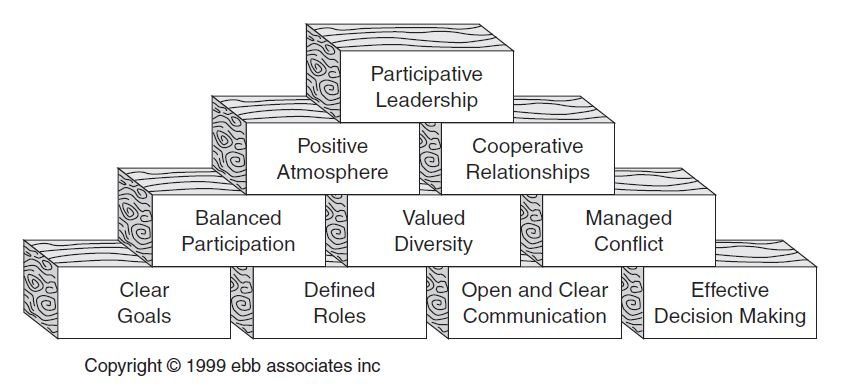
\includegraphics[scale=0.9]{Abbildungen/Ten_Characteristics.JPG}\\
			\caption[Abbildung 1]{Ten Characteristics of a High Performance Team \citep[p. 27]{biech2007pfeiffer}}
			\label{ten_characteristics}
		\end{footnotesize}
	\end{figure}
	Die einzelnen Teilbereiche bauen aufeinander auf. Der untere Teilbereich mit den Komponenten \textit{Clear Goals"}, \textit{Defined Roles}, \textit{Open and Clear Communication} sowie \textit{Effective Decision Making} sind die Basis des gesamten Models. Diese Komponenten sollten am Anfang des Teambuildingprozesses definiert und immer als Basis der gesamten Teamarbeit gesehen werden.\\
	Der Teilbereich mit den Komponenten \textit{Balanced Participation}, \textit{Valued Diversity} und \textit{Managed Conflict} baut auf diese auf.\\
	\textit{Positive Atmosphere} und \textit{Cooperative Relationships} ist der dritte Teilbereich. In diesem geht es hauptsächlich um die Zufriedenheit und die Bereicherung eines einzelnen in einem Team zu arbeiten. Jedoch ist dieser Bereich nicht mehr Ausschlaggebend um eine Aufgabe zu erledigen. Für viele Teammitglieder ist dieser Teilbereich jedoch wichtigste Ziel während der Teamarbeit.\\
	\textit{Participative Leadership} ist der einzige Bereich der aus dem Gesamtgebilde ohne Beeinflussung der anderen Komponenten entfernt werden kann. Dies sagt uns, dass ein Teamm auch ohne einen einzelnen Teamleiter existieren kann. Vgl. \citep[p. 13-16]{biech2007pfeiffer}\\
	Aufgrund der vielen Komponenten die ein Team erfüllen muss um effizient zu sein und ein Gestärktes Teamgefühl zu bilden, wird in dieser Ausarbeitung nur auf einen Teilbereich eingegangen.
	
	\paragraph{Positive Atmosphere}
	Wird der Aufbau von Vertrauen vernachlässigt, so bildet sich kein gut funktionierendes Team.
	\paragraph{Open and Clear Communication}
	\paragraph{Balanced Participation}
	\paragraph{Defined Roles}
	
		\subsubsection{Team-Colloboraton}
		\subsubsection{Virtual-Teambuilding}
		
		\paragraph{Allgemeines}
		Virtuelle Teams werden häufig gebildet um räumliche oder kurzzeitige Trennungen eines Teams zu umgehen. Dabei werden computergestützte Technologien verwendet. \citep[p. 1-2]{cascio2003leadership}
		
		Virtuellen Teams ist es möglich, dass räumlich getrennte Teammitglieder ihre Aufgaben, mittels computergestützter Kommunikation, im Team koordinieren können. \citep[p. 117-119]{peters2007identifying} \textbf(117,118,119 - Seitenzahl nicht sicher :) )
		
		Es kann effizient Länderübergreifend gearbeitet werden, was ein größeres Innovationspotential für Unternehmen zur folge hat.	
		Virtuelle Teams haben den Ruf teuer zu sein, die Ziele nicht verfolgen zu können, nie pünktlich und schwierig zu managen zu sein. \citep[p. 243-244]{gassmann2003trends}
		
		Virtuelle Teams sind häufig -gerade in der Anfangsphase- sehr Ergebnisorientiert in der Art und Weise \textit{wie} kommuniziert wird. Dieses Defizit in der Sozialen Kommunikation untereinander kann die Schlüsselfaktoren eines Erfolgreichen Teams beeinträchtigen - Soziale und Emotionale Beziehungsbildung sowie den Aufbau von Vertrauen. \citep[p.378]{ren2007applying} \\
		Um die Wahrscheinlichkeit zu erhöhen, dass auch in der Anfangsphase des Teambuildings eine \glqq Soziale\grqq und keine \glqq Arbeitsnahe, Ergebnisorientierte\grqq Kommunikation stattfindet, wurde das "Escape-Room-Artige" Szenario gewählt um den Teilnehmern eine spielerische Umgebung zu schaffen. 
		
		\paragraph{Social Identity}
		Personen fühlen sich zu einer Vielzahl von Gruppen hingezogen. Das Soziale Identitätsgefühl hängt davon ab, ob ein generelles Gruppenverständnis besteht, eine Person sich der Gruppe zugehörig fühlt und ob man sich zu als Gruppe mit anderen Gruppen vergleicht. Gruppenzugehörigkeit ist ein wichtiger Bestandteil des Selbstverständnisses eines Individuums. \citep{sutantovicious}
		Ist gute Gruppenzugehörigkeit gegeben, stärkt dies die Gruppenproduktivität sowie die individuelle Leistungsfähigkeit. Weiterhin entstehen dadurch Effekte die zum besserem Zusammenhalt, mehr Vertrauen \citep{herbsleb2000distance}, besserer Kommunikation und Kooperation untereinander führen. \citep[p. 510]{olson2003psychological}
		
		
		\subsubsection{Vorteile/Nachteile von Teambuilding}
		
		\section{Trust}
		\subsection{Cognitive Trust}
		\subsection{General-Trust}
		
	\newpage
	\section{Versuchshypothesen}
		\paragraph{Head- und Handtracking ohne Inversekinematisch-simulierten-Torso steigert das Vertrauen in den Gegenüber mehr als Head,-Hand und mit Inversekinematisch-simulierten-Torso.}
		\paragraph{Es findet mehr Kommunikation ohne Inversekinematisch-simulierten-Torso statt als mit Inversekinematisch-simulierten-Torso.}
		\paragraph{Es existiert ein größeres Zusammenhaltsgefühl ohne Inversekinematisch-simulierten-Torso als mit Inversekinematisch-simulierten-Torso.}
		
	\section{Vorgehensweise}
		\subsection{Verwendete Technik}
			\subsubsection{Verwendete Hardware}
			\subsubsection{Verwendetes Framework}
		\subsection{Zielgruppe}
		Die Voraussetzung um an dem Versuch Teilzunehmen, ist es, ein \ac{HDM}, zwei Controller sowie ein Computer mit Internetzugang zu besitzen. Der gesamte Versuch ist als ein "Into the Wild" Versuch aufgebaut, welches bedeutet, dass die genaue Zielgruppe nicht genau definiert werden kann. Die einzigen Ristriktion sind die vorher beschriebenen Konditionen. 
		\subsection{Untersuchungsmethode}
			\subsection{Qualitative vs Quantitative Untersuchung}
			\subsubsection{A/B Testing}
			\subsubsection{Teilnehmerfindung}
			\subsubsection{Datenerhebungsmethoden}
				\paragraph{Fragenbogen}
				Es werden zwei Fragenbögen an die jeweiligen Studienteilnehmer verteilt. Der erste Fragenbogen wurde an die Probanten vor der eigentlichen Studie ausgefüllt. Ziel war es, die Einstellungen zu Teamarbeit sowie zu Interpersonellem Vertrauen der Personen vor der eigentlichen Untersuchung festzustellen. Der Zweite Fragebogen wurde nach der Untersuchung ausgefüllt, um die Effektivität der verschiedenen Konditionen der Untersuchung auf Erfolg oder Misserfolg untersuchen zu können.
				Es wurden nur vollständig Ausgefüllte Fragebögen zur Datenanalyse herangezogen. Konnte nicht ermittelt werden, welche Aussage angekreuzt wurde, wurde dieser ebenfalls nicht mit in die Datenanalyse aufgenommen. Eine Außnahme war dabei, falls ein Teilnehmer im Nachhinein nach die von Ihm gewünschte Antwort befragt werden konnte.
				\paragraph{Beobachtung}
				Durch die Beobachtung während des Experiments werden Kennzahlen zur Dauer des Versuchs zwischen den einzelnen Konditionen bestimmt. Anhand dieser kann im späterem Verlauf das  Teambuilding Potential sowie die subjektive Effektivität durch gesteigertem Swift-Trust analysiert werden.
				\paragraph{Induktive Quantitative Forschungsmethodik}
				Anhand der subjektiven Betrachtungsweise einzelner Personen des Themas "Vertrauen" wurde ein quantitatives Forschungsdesign gewählt anhand die Ergebnisse induktiv interpretiert und ausgewertet wurden.
		\subsection{Abhängige Variablen}
			\subsubsection{Generelles Vertrauen}
			Wie in \textbf{Abbildung \ref{ten_characteristics}} beschrieben \textbf{ABBILDUNG 1 BESCHREIBEN, TRUST z.B. UND EINZELNE PUNKTE}, ist die Positive Atmosphere in einem Team einer der Maßgeblichen Faktoren die zur Leistungsfähigkeit und zum \textit{\glqq wir-gefühl\grqq} beitragen.
			Die Abhängige Variable Vertrauen ...	
			%\paragraph{Swift-Trust}
			%\subsubsection{Kommunikation}
			%\subsubsection{Team Zusammenhalt}
			%\subsubsection{Teambuilding Potential}
			\subsubsection{Vertrauen in das Team}
			\subsubsection{Team Effektivität}
			%\subsubsection{Andere Faktoren}
		\subsection{Unabhängige Variablen}
			\subsubsection{Avatar embodiement}
				\paragraph{Head- and Handtracking}
				\paragraph{Head-,Hand and Inversekinematic-Torso}
		\subsection{Residuen}
			\subsubsection{Aufbau der Umgebung}
			\subsubsection{Sozialpsychologische Einflussfaktoren}
				\paragraph{Gamification} $~$ \\
				\paragraph{Aussehen} $~$ \\
				\paragraph{Sprache} $~$ \\	
				\paragraph{Bekanntheit}
				Um die gegenseitige Bekanntheit der Probanten auszuschließen, wurde jedem Probanten zu beginn des Versuchs ein Zufälliger anonymer Name zugeordnet.
		\subsection{Beschreibung des Forschungsverlaufs}
		Insgesamt nahmen \textbf{ANZAHL DER TEILNEHMER} am Versuch teil.
		Jeder Probant bekam einen zufälligen Zeitslot sowie ein anonymen Namen zugeordnet mit dem dieser an dem Versuch teilnahm. Gemäß des A/B-Testings wurden jeweils drei Personen in einem Zeitslot untergebracht um ein "Team" zu bilden. Diesem "Team" wurde entweder die Kondition "Head- und Handtracking" oder "Head-, Hand mit Inversekinematisch-simulierten-Torso" zugeordnet. Somit nahmen drei Probanten, am selben Versuch zur selben Zeit mit der selben Kondition, teil. Die Probanten wurden nicht Face-To-Face vorgestellt und sahen sowie hörten sich während des gesamten Versuchs nur als Repräsentation eines Avatars in der Virtuellen Umgebung. Der Zeitslot von 30 Minuten teilte sich auf in
		\begin{itemize}
			\item 10 Minuten Pre-Questionnaire
			\item 20 Minuten Versuchsdurchführung
			\item 10 Minuten Post-Questionnaire
		\end{itemize}
		Jeder Teilnehmer bekam zu beginn seines Zeitslots einen Fragebogen, den dieser selbstständig ausfüllen sollte. Dieser wurde von \textbf{ANZAHL DER PERSONEN} Personen ausgefüllt. \textbf{Da nicht alle Fragebögen vollständig ausgefüllt wurden, konnten nur X Ergebnisse in die Analyse mit eingezogen werden.}
		Nachdem alle Probanten den Fragebogen ausgefüllt haben, begann das Experiment. Dazu loggte sich das jeweilige Team in das \ac{SVE} ein und spielten den Versuch durch.
		Während des Experiments wurden Notizen zum Verhalten der einzelnen Personen gemacht um herauszufinden, ob beispielsweise einer die Teamleaderrolle übernimmt, in welchem Maß interpersonelle Kommunikation stattfindet oder wie die Teilnehmer auf die jeweiligen Avatare reagieren.
		Als das Team mit dem Experiment fertig war, wurde ein weiterer Fragebogen ausgeteilt um verschiedene Faktoren nach dem Experiment analysieren zu können. Dieser wurde von \textbf{ANZAHL DER PERSONEN} Personen ausgefüllt. \textbf{Da nicht alle Fragebögen vollständig ausgefüllt wurden, konnten nur X Ergebnisse in die Analyse mit eingezogen werden.}
		
		\subsection{Der Versuchsaufbau}
		
	\newpage
	\section{Ergebnisse}
		\subsection{Validität und Reliabilität}
		Weshalb ist meine Forschung Valide? Weshalb ist sie reliabel?	
		\textit{BEISPIEL : Die Forschung ist valide, da immer dieselbe Waage verwendet wurde, die exakt nach europäischen Standards wiegt. Zudem wurde die Reliabilität der Waage während der Untersuchung täglich getestet, indem ein Kilogramm Blei darauf gelegt wurde. Jedes Mal zeigte die Waage dabei ein Kilo an.}
		\subsection {Gesammelte Daten}
	
		\subsection{Analyse}
	\newpage
	\section{Zusammenfassung}
	\newpage
	\section{Diskussion}
		\subsection{Diskussion der Ergebnisse}
		\subsection{Diskussion der eingesetzten Methoden}
		\subsection{Auswirkungen auf die Gegenwart}
		\subsection{Vorschläge für zukünftige Untersuchungen}
	
	\newpage
	\appendix	
	\section*{Anhang}\markboth{Anhang}{Anhang}\addcontentsline{toc}{section}{Anhang}
	Den Anhang beginnen Sie auf einer neuen Seite und in einem neuen Abschnitt. Die Überschrift selbst wird nicht nummeriert.
	\newpage

\bibliographystyle{dcu}
\bibliography{bibfile}
\end{document}